\chapter{Introducción}
 En este capítulo se detalla la motivación que llevó a la realización del proyecto, los objetivos que este comprende y las pautas que se tomaron para lograr llevarlo a cabo
    
    \section{Objetivo}
    
    Este Trabajo de Final de Grado busca la implementación de un portal web que permita la recopilación de datos de interés para el estudio por parte del equipo médico. Para ello contará con formularios personalizados con los campos de interés  solicitados por el mismo que serán rellenados por los médicos en consultas rutinarias con los pacientes que hayan consentido participar en el proyecto. Estos datos serán luego accesibles tanto vía web como en archivos de Excel descargables desde el propio portal.\newline

	Con el fin de ajustar el producto final a las necesidades del equipo la aplicación se entregará con tiempo suficiente (aproximadamente en febrero de 2020) para que pueda ser probada, revisada y modificada a medida. Esto es especialmente importante ya que el estudio se extenderá muchos meses más allá de la finalización de este TFG.\newline

	El objetivo final, y por supuesto el más importante, es que todo este desarrollo sirva de herramienta para ajustar los criterios de evaluación en los pacientes con diabetes mellitus tipo 2, permitiendo encontrar pautas en sus estados de salud subsanables que puedan en un futuro prevenir más casos de esta enfermedad.\newpage
	
	\section{Motivación}
    
    Nuestra primera motivación para adentrarnos en este proyecto son las tecnologías empleadas en el mismo. Ambos participantes estamos interesados en centrar nuestras carreras en tecnologías web, uno de ellos trabajando ya de hecho como desarrollador \textit{full-stack}. El proyecto da además libertad para ser implementado sin ningún tipo de restricciones de diseño o rendimiento, lo que plantea un escenario ideal para experimentar durante su desarrollo.\newline

	El otro motivo principal para decantarnos por este proyecto es su cercanía a un proyecto real. El cliente, la aplicación, los plazos y las necesidades del mismo no son algo creado para un ambiente académico, como otros desarrollos ya efectuados durante la carrera, sino un problema real que precisa una solución efectiva contando con todas las personas que lo acabarán utilizando. Además el proyecto requerirá de un mantenimiento post entrega, otro ámbito nunca explorado en la carrera y que será una valiosa experiencia de cara a nuestro futuro.\newline

	Por último remarcar que uno de los miembros, Sergio, ya tiene buenas experiencias con un proyecto anterior para el ámbito médico desarrollado en solitario para una empresa en Suiza y Eduardo siempre ha tenido interés en los hábitos de vida saludables y la nutrición, posible principal remedio para la diabetes extraído de los resultados de este estudio.\newpage
	
	\section{Metodología de trabajo}
    
    El proyecto será planificado bajo los estándares de la metodología Scrum\cite{Scrum} aunque distendiendo un poco sus cotas temporales, pues al ser solo dos miembros no es necesario hacer un hincapié tan diario en la organización para mantener el orden. Lo primero será definir cómo mantendremos los tres pilares básicos de la metodología: \textbf{transparencia, inspección y adaptación}.
    
    \begin{figure}[h]
    \centering
     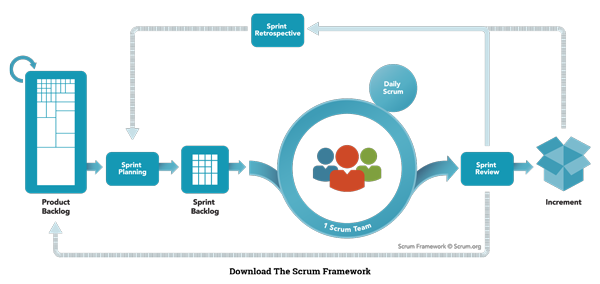
\includegraphics[width=1\textwidth]{images/Scrum.png}
    \caption{Flujo de trabajo en Scrum. Imagen obtenida de Scrum.org \cite{Scrum.org}}
    \end{figure}
    
    \subsection{Transparencia}
    Para mantener a ambos miembros al día de cualquier avance o variación en el proceso se empleará la herramienta online de Trello\cite{Trello}, que nos permitirá ir viendo en tiempo real los mismos. Este será estructurado de la siguiente forma:
    
    \begin{itemize}
    \item Se crearán dos columnas, una con la lista de tareas pendientes para el sprint actual y otra con las tareas actualmente en desarrollo. Además se creará una columna por cada sprint en la que se irán almacenando todas las tareas finalizadas. Cada tarea podrá encapsularse en una o más de estas categorías: despliegue, documentación, front, bug, investigación, modelo de datos, pendiente de resolver (cuestión a espera de la próxima reunión con el tutor), back, varios, resuelto (cuestiones ya solucionadas en anteriores reuniones que quedan como recordatorio). Además cada tarea llevará una o más etiquetas indicando los desarrolladores que han trabajado en ella.\newline
    
     \begin{figure}[h]
    \centering
     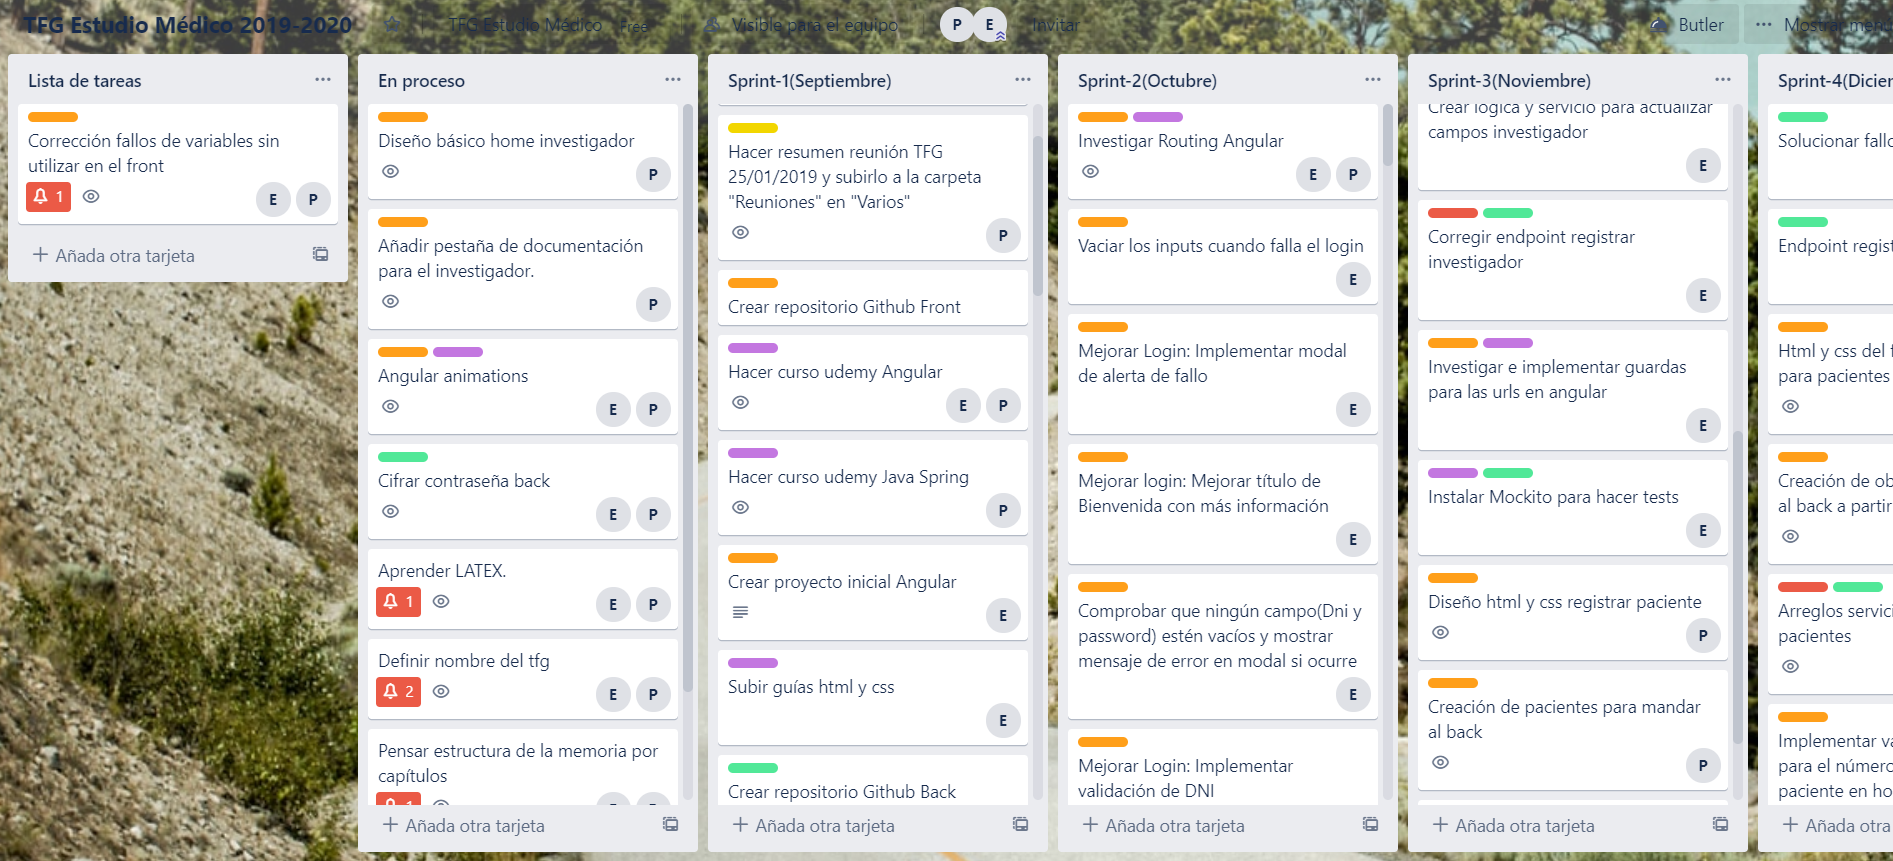
\includegraphics[width=1\textwidth]{images/Trello.jpg}
    \caption{Captura de ejemplo de la herramienta Trello.}
    \end{figure}
    \newpage
    
    \item  Asimismo, todo el código del proyecto estará subido y actualizado en un repositorio, en este caso GitHub\cite{github}, a través del cual se podrá ver un histórico preciso de los cambios realizados en cada \textit{commit} junto a comentarios explicativos del desarrollador que los haya realizado.\newline
    
    \begin{figure}[h]
    \centering
     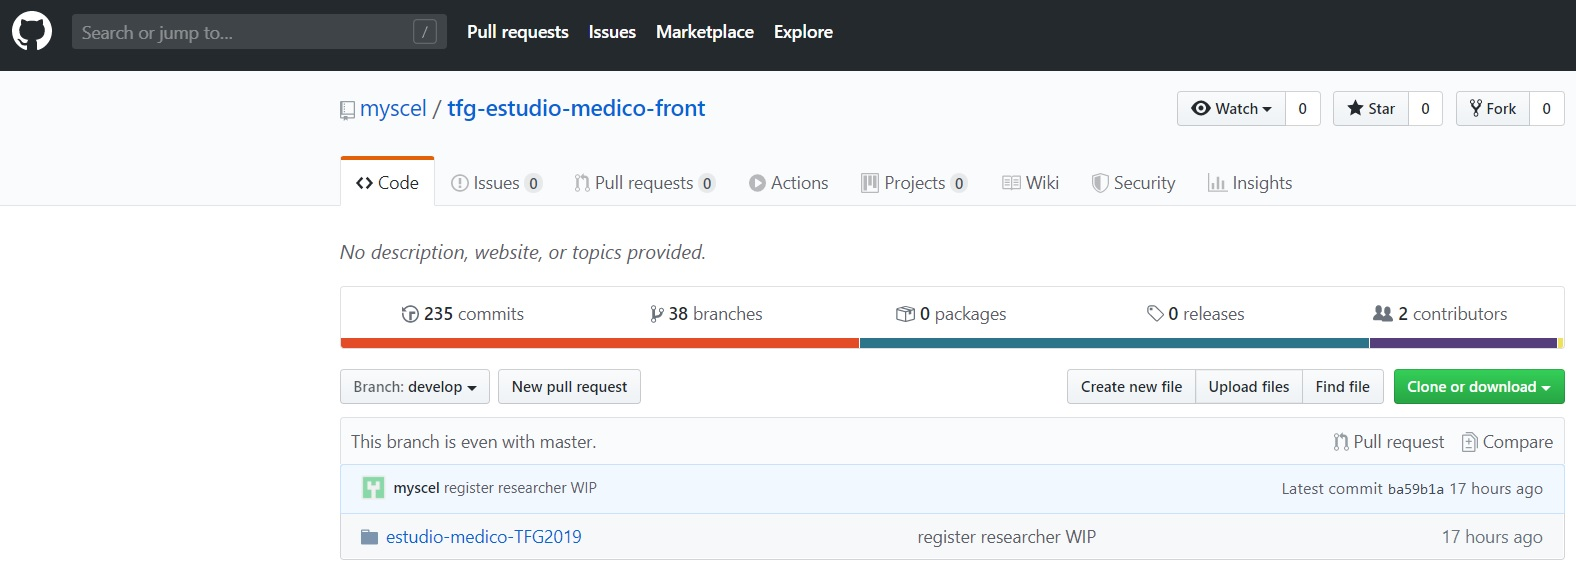
\includegraphics[width=1\textwidth]{images/GitHubFront.jpg}
    \caption{Captura de ejemplo del repositorio front en GitHub.}
    \end{figure}
    \end{itemize}
    
    \subsection{Inspección}
    Con el fin de mantener este principio, nuestro repositorio no solo albergará código, sino también un espacio separado para todos los artefactos derivados de Scrum, así como la documentación que se vaya creando durante el proceso que sea relevante a efectos de esta memoria. Estos artefactos serán por tanto accesibles constantemente por ambos miembros, los cuales avisarán en caso de cualquier añadido o modificación para que su compañero pueda revisarlo.\newline
    
    \begin{figure}[h]
    \centering
     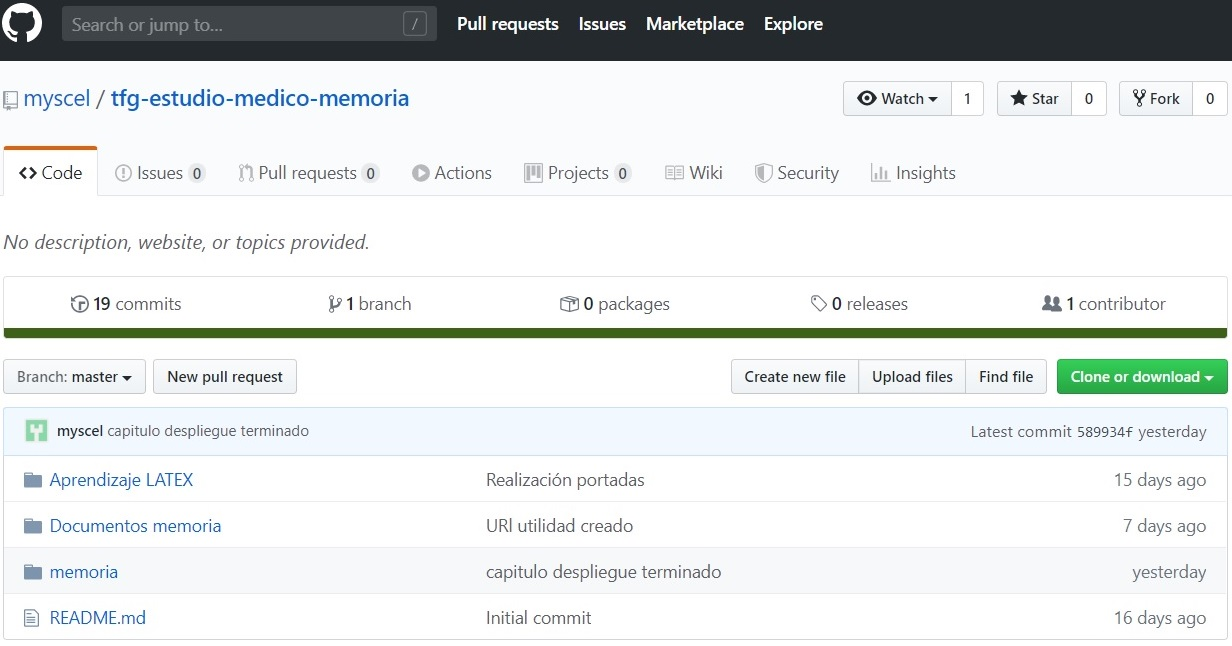
\includegraphics[width=1\textwidth]{images/GitHubMemoria.jpg}
    \caption{Captura de ejemplo con todos los documentos referentes a la memoria en GitHub tomada a posteriori.}
    \end{figure}
    \newpage
    
     \subsection{Adaptación}
    Al final de cada sprint se realizará una reunión tanto con el tutor del proyecto como con un representante del equipo médico para revisar el proceso y obtener \textit{feedback} del mismo. Los errores o cambios urgentes extraídos de estas reuniones pasarán a ser la tareas más prioritarias del proyecto y su resolución será notificada de inmediato a ambos asistentes de la reunión. Además, para mantener el proyecto lo más afín a las necesidades del cliente cualquier cambio significativo en mitad de un \textit{sprint} será notificado por correo previamente.
    \newline
    
    Además, de toda la documentación y artefactos mencionados disponibles durante el desarrollo los miembros mantendrán un contacto diario hablando de qué se ha hecho, se va a hacer y los problemas que se van encontrando, el cual hará las veces de \textit{Daily Scrums}.\newline

	En cuanto a los roles típicos de Scrum, en nuestro caso, no serán utilizados. El \textit{Product Owner} será suplido con la comunicación directa y constante  de los miembros con el cliente que asegurará la priorización del valor para este durante el desarrollo. El \textit{Scrum Master} no será preciso ya que ambos miembros del equipo tienen experiencia utilizando metodologías ágiles, tanto en la carrera como fuera en trabajos o proyectos propios. Por tanto solo existirá el equipo de desarrollo y este suplirá las funciones necesarias del resto de roles.\newline

	Los \textit{sprints} serán de una duración mensual. Se opta por esta cuantía porque al estar uno de los miembros aún con clases y otro trabajando a jornada completa no se estima que en una semana el desarrollo pueda tener un avance suficientemente significativo. Estos sprints se iniciarán con una reunión de planificación con el tutor del proyecto y el representante del equipo médico, estipulando qué se hará y cómo. Asimismo, concluirán con otra reunión de misma índole que mostrará una demo funcional al representante y recogerá su \textit{feedback}, para acto seguido comenzar con la reunión de planificación del siguiente \textit{sprint}. Se decide aunar así el inicio y final del sprint en una sola reunión para evitar problemas de horarios difíciles de encajar por parte de los cuatro. Tras esta reunión con todos los miembros se realizará una pequeña reunión de retrospectiva solo del equipo de desarrollo para determinar si la metodología de trabajo funciona y qué se podría modificar o añadir.\newline

\chapter*{Introduction}
\addcontentsline{toc}{chapter}{1. Introduction}
This chapter details the motivation that led to the realization of this project, the objectives that it comprises and the guidelines that were taken to achieve it.


    \section*{1.1. Objective}
    \addcontentsline{toc}{section}{1.1. Objective}
    
    This Final Degree Project seeks the implementation of a web portal that allows the collection of data of interest for the study of the medical team. To do this, it will have personalized forms with the fields of interest requested by them, which will be filled in by doctors in routine appointments with patients who have consented to participate in the project. These data will then be accessible both via the web and in a downloadable Excel file from the portal itself.\newline
	
    In order to adjust the final product to the needs of the team, the application will be launched with 
    enough time (approximately in February 2020) so that it can be tested and modified to measure. This is especially important since the study will extend many months beyond the end of this FDP.\newline
	
	The final objective, and of course the most important one, is that all this development serves as a tool to adjust the evaluation criteria in patients with type 2 diabetes mellitus, allowing to find guidelines to improve in their life habits that may prevent more cases of this disease in the future.\newpage
	
	\section*{1.2. Motivation}
    \addcontentsline{toc}{section}{1.2. Motivation}
    
    Our first motivation to get into this project is the technologies used in it. Both participants are interested in focusing their career on web technologies, in fact one of them is already working as a full-stack developer. The project also gives freedom to be implemented without any design or performance restrictions, which presents an ideal scenario to experiment during its development.\newline
	
	The other main reason for opting for this project is its proximity to a real project. The client, the application, the deadlines, and the needs of this project are not something created for an academic environment, like other developments already carried out during the degree, but a real problem that requires an effective solution with all the people who will end up using it. In addition, the project will require post-launch maintenance, another area never explored in the degree and which will be a valuable experience for our future.\newline
	
	Note that one of the members, Sergio, already has good experiences with a previous project in the medical field developed alone for a Switzerland company, and Eduardo has always had an interest in healthy lifestyle habits and nutrition, possible main remedy for diabetes extracted from the results of this study.\newpage

	\section*{1.3. Work methodology}
    \addcontentsline{toc}{section}{1.3. Work methodology}
    
    The project will be planned under the standards of the Scrum\cite{Scrum} methodology, although it will slightly loosen its temporary limits. Since there are only two members it is not necessary to place such daily emphasis on the organization to maintain order. The first thing will be to define how we will maintain the three basic pillars of the methodology: \textbf{transparency, inspection and adaptation}.
    
    \begin{figure}[h]
    \centering
     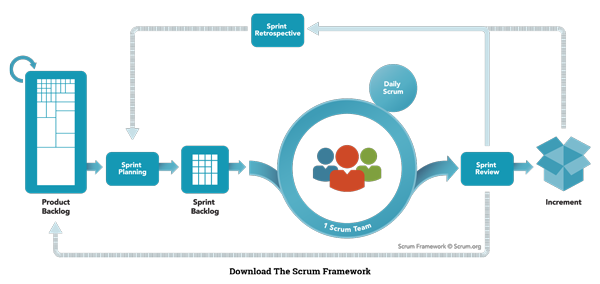
\includegraphics[width=1\textwidth]{images/Scrum.png}
    \caption{Workflow on Scrum. Picture obtained from Scrum.org \cite{Scrum.org}}
    \end{figure}
    
    \subsection*{1.3.1. Transparency}
    \addcontentsline{toc}{subsection}{1.3.1. Transparency}

    To keep both members up to date with any progress or variation in the process we will be using Trello's\cite{Trello} online tool, which will allow us to see them in real time. This will be structured in the following way:
    
    \begin{itemize}
    \item Two columns will be created, one with the list of pending tasks for the current sprint, and another with the tasks currently in progress. In addition, a column will be created for each sprint in which all the completed tasks will be stored. Each task can be encapsulated in one or more of these categories: deployment, documentation, FrontEnd, bug, research, data model, pending resolution (questions for the the next meeting with the tutor), BackEnd, variety, resolved (questions already solved in previous meetings that stay as a reminder). Also, each task will have one or more labels indicating the developers who have worked on it.\newline

    
     \begin{figure}[h]
    \centering
     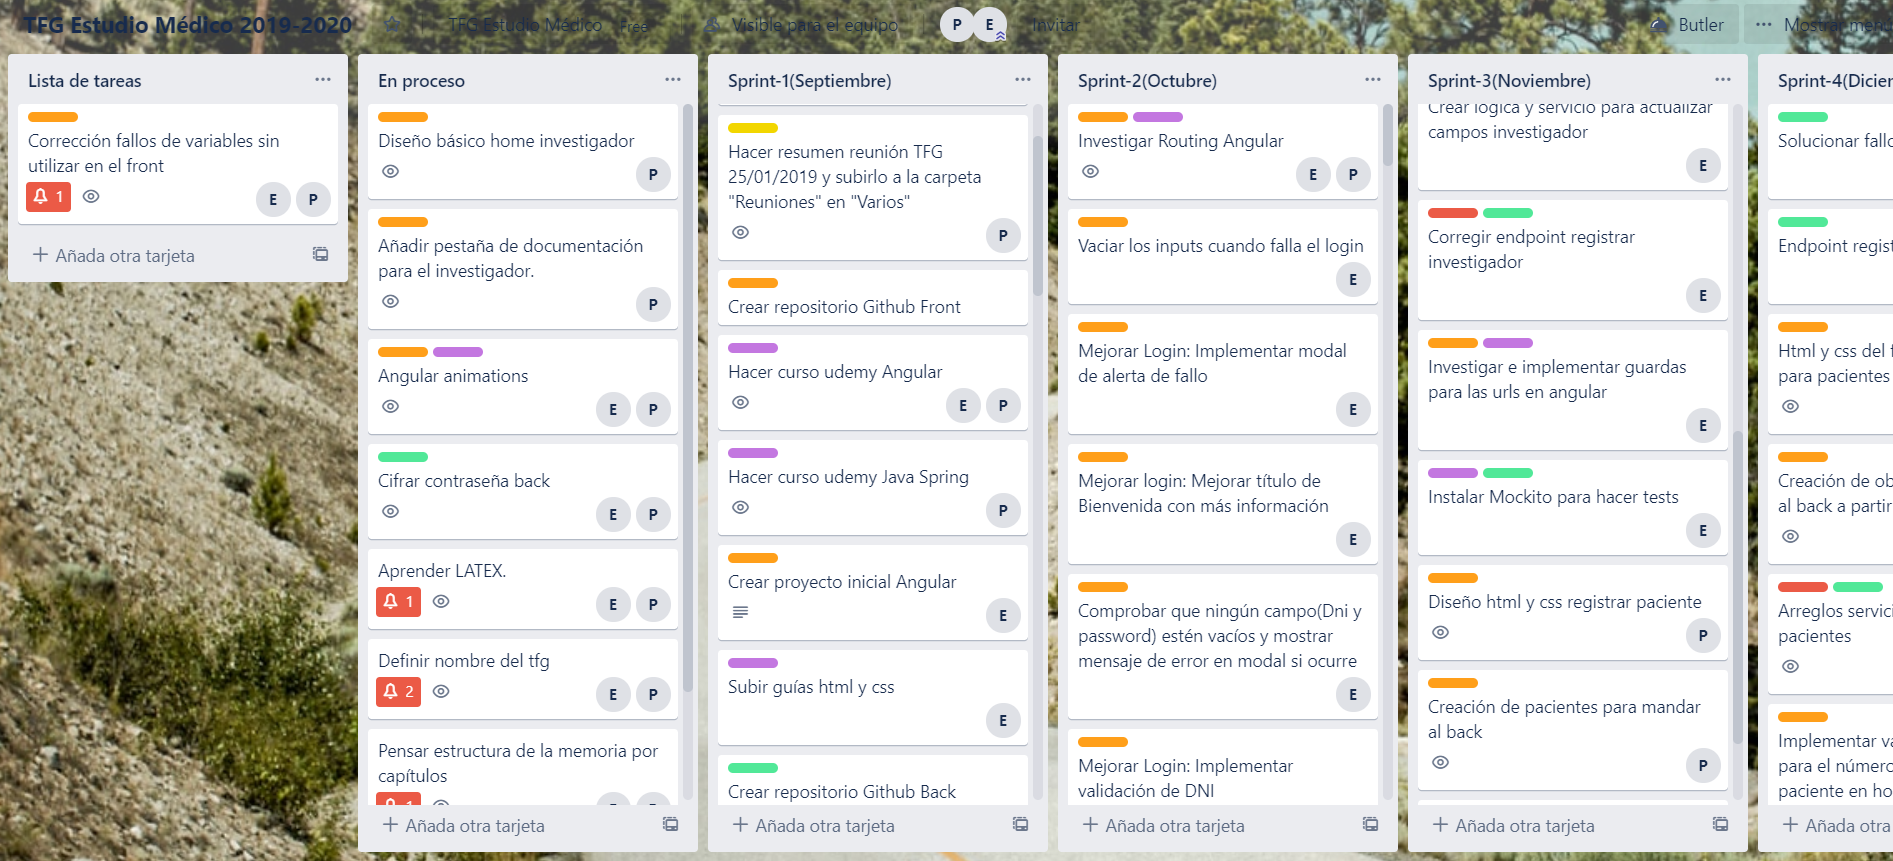
\includegraphics[width=1\textwidth]{images/Trello.jpg}
    \caption{Example image of Trello's online tool.}
    \end{figure}
    \newpage
    
    \item  Also, all the project code will be uploaded and updated in a repository, in this case GitHub\cite{github}, through which you can see an accurate history of the changes made in each commit along with explanatory comments from the developer that realised them.\newline

    \begin{figure}[h]
    \centering
     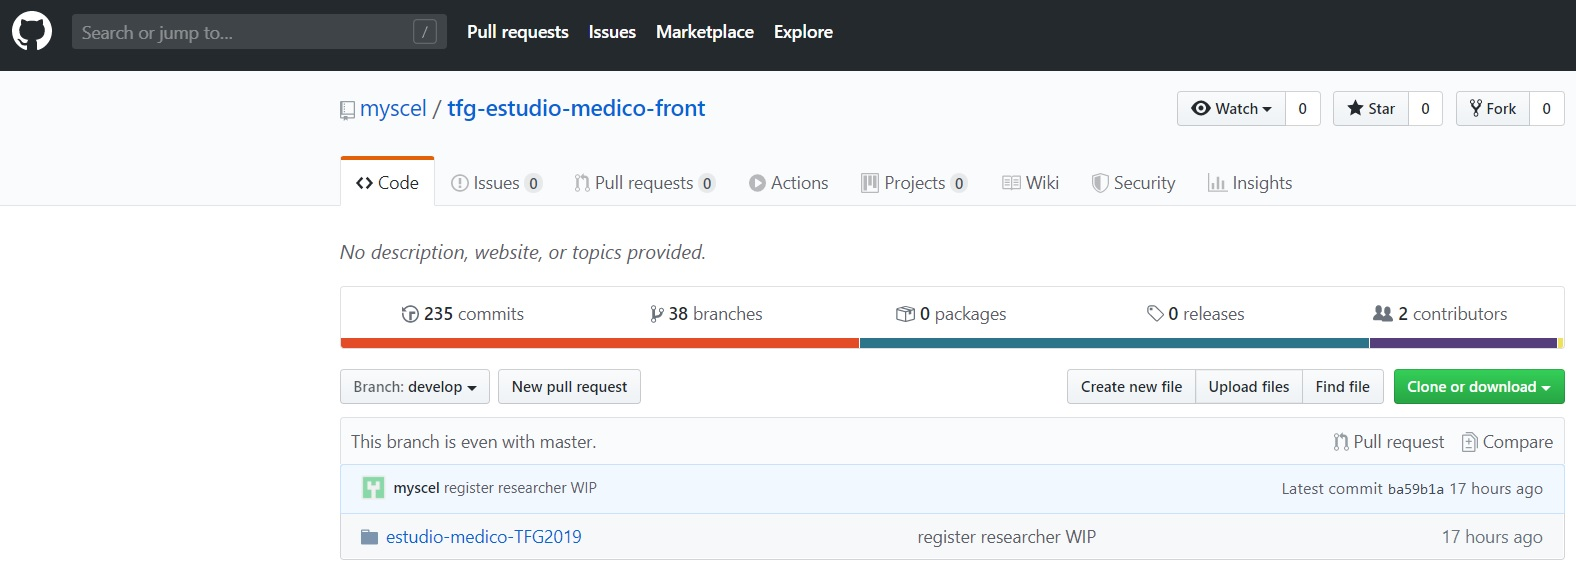
\includegraphics[width=1\textwidth]{images/GitHubFront.jpg}
    \caption{Example image of FrontEnd repository on GuitHub.}
    \end{figure}
    \end{itemize}
    
    \subsection*{1.3.2. Inspection}
    \addcontentsline{toc}{subsection}{1.3.2. Inspection}
    In order to uphold this principle, our repository will not only store code, but also a separate space for all the artifacts derived from Scrum, as well as the documentation that is created during the process that is relevant for the purposes of this report. These artifacts will therefore be constantly accessible by both members, who will notify in case of any addition or modification so that their partner can review them.\newline
    
    \begin{figure}[h]
    \centering
     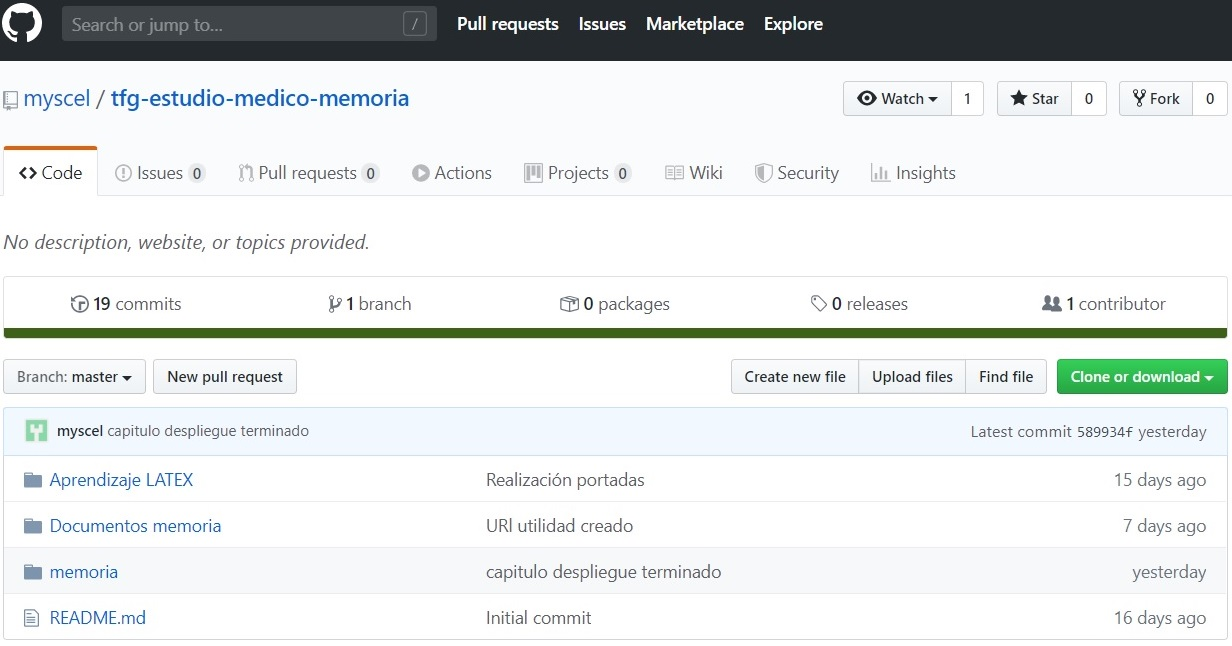
\includegraphics[width=1\textwidth]{images/GitHubMemoria.jpg}
    \caption{Example image of all the documents about this report on GitHub.}
    \end{figure}
    \newpage
    
     \subsection*{1.3.3. Adaptation}
    \addcontentsline{toc}{subsection}{1.3.3. Adaptation}
    
    At the end of each sprint there will be a meeting with both the project tutor and a representative of the medical team to review the process and obtain feedback on it. Errors or urgent changes extracted from these meetings will become the highest priority of the project and their resolution will be immediately notified to both meeting attendees. In addition, to keep the project as close as possible to the client's needs, any significant change in the middle of a sprint will be notified by mail in advance to them.\newline
    
    In addition of all the documentation and artifacts mentioned available during the development, the members will keep a daily contact talking about what has been done, what is going to be done and the problems they are encountering, which will act as Daily Scrums.\newline
	
	As for the typical Scrum roles, in our case, they will not be used. The Product Owner will be replaced with the direct and constant communication of the members with the client that will ensure the prioritization of the most valuable features for him during the development. The Scrum Master will not be precise since both team members have experience using agile methodologies, both in the career and outside in their own work or projects. Therefore, only the development team will exist and this will supply the functions for the rest of the roles.\newline
	
	Sprints will be monthly. This amount is chosen because one of the members is still with classes and the other is working full time. It is not estimated that in one week the development can have a  significant advance. These sprints will begin with a planning meeting with the project tutor and the medical team representative, stipulating what will be done. Likewise, they will conclude with another meeting of the same nature that will show a functional demo to the representative and collect their feedback, to then begin with the planning meeting for the next sprint. It was decided to combine the start and end of the sprint in a single meeting in order to avoid problems with schedules that were difficult for all four to fit into. After this meeting with all the members there will be a small retrospective meeting only for the development team to determine if the work methodology works and what could be modified or added.